\documentclass[twocolumn, 10pt]{article}
\usepackage{ctex}
\usepackage{amsmath}
\usepackage{amsfonts}
\usepackage{amssymb}
\usepackage{graphicx}
\usepackage{float}
\usepackage{listings}
\usepackage{color}
\usepackage{geometry}
\usepackage{fancyhdr}
\usepackage{titlesec}
\usepackage{tikz}
\usepackage{pgfplots}
\usepackage{pgfplotstable}
\usepackage{booktabs}
\usepackage{caption}
\usepackage{subcaption}
\usepackage{algorithm}
\usepackage{multirow}
\usepackage{array}
\usepackage{enumitem}
\usepackage{hyperref}
\usepackage{svg}
\usepackage{fontspec}
\usepackage{algpseudocode}
\usepackage[table]{xcolor}

\graphicspath{{img/}}
\renewcommand\arraystretch{1.2}
\newcommand{\figureBelowMargin}{\vspace{-2pt}}
\newcommand{\kea}{K{\small\MakeUppercase{ea}}}
\newcommand{\lamp}{L{\small\MakeUppercase{amp}}}
\geometry{a4paper,scale=0.8}
\title{\fontspec{Times New Roman} LAMP: Large-language-model Augmented Mobile Testing Path Exploration Based on Kea}

\author{
  Group 07\\
  李鹏达$^{*}$, 武泽恺$^{\dagger}$, 张耘彪$^{\ddagger}$\\
  \texttt{10225101460}$^{*}$, 
  \texttt{10225101429}$^{\dagger}$, 
  \texttt{10225101437}$^{\ddagger}$
}
\date{}

\lstset{
    % language = C,
    xleftmargin = 3em,xrightmargin = 3em, aboveskip = 1em,
	backgroundcolor = \color{white}, % 背景色
	basicstyle = \small\ttfamily, % 基本样式 + 小号字体
	rulesepcolor= \color{gray}, % 代码块边框颜色
	breaklines = true, % 代码过长则换行
	numbers = left, % 行号在左侧显示
    numberstyle = \small, % 行号字体
    numbersep = -14pt, 
    keywordstyle=\color{purple}\bfseries, % 关键字颜色
    commentstyle =\color{red!50!green!50!blue!60}, % 注释颜色
    stringstyle = \color{red}, % 字符串颜色
    morekeywords={ASSERT, int64_t, uint32_t},
	frame = single, 
	showspaces = false, % 不显示空格
    showstringspaces = false,
	columns = fixed, % 字间距固定
    literate=
        {^-}{{{\color{black}\textbf{\color{red}-}}\colorbox{red!30}{\phantom{XX}}}}{1}
        {^+}{{{\color{black}\textbf{\color{green}+}}\colorbox{green!30}{\phantom{XX}}}}{1},
}

\begin{document}

\maketitle

\section{背景}

移动应用自动化测试是目前正在快速发展的领域,研究热点包括UI引导的测试输入生成、基于属性的测试(Property-Based Testing,PBT)、大语言模型(Large Language Model,LLM)的应用以及上下文感知的文本输入生成等技术方向。DroidBot\cite{li2017droidbot}等UI引导的测试工具通过动态构建状态转移模型,生成高效的测试输入,适用于兼容性测试和安全分析;基于属性的测试\cite{xiong2024general}通过定义功能属性并生成输入事件序列,有效检测非崩溃性功能错误;InputBlaster\cite{liu2024testing}, QTypist\cite{liu2023fill} 和 GPTDroid\cite{liu2024make} 等工具利用大语言模型的语义理解和生成能力,在异常输入生成、文本输入生成、测试脚本生成和Bug复现等方面表现出色,显著提升了测试覆盖率和错误检测能力;上下文感知的文本输入生成技术\cite{liu2023fill}则通过提取GUI上下文信息,生成符合语义的输入,填补了文本输入测试的空白。这些技术在移动应用测试中取得了显著的进展。

其中, \kea\cite{xiong2024general}是一个基于属性测试的移动应用测试工具。它将基于属性的测试引入移动应用测试,通过定义功能属性并结合路径探索,发现Android应用中的非崩溃性功能错误,提供了更深入的功能验证能力。

\begin{figure}[ht!]
    \centering
    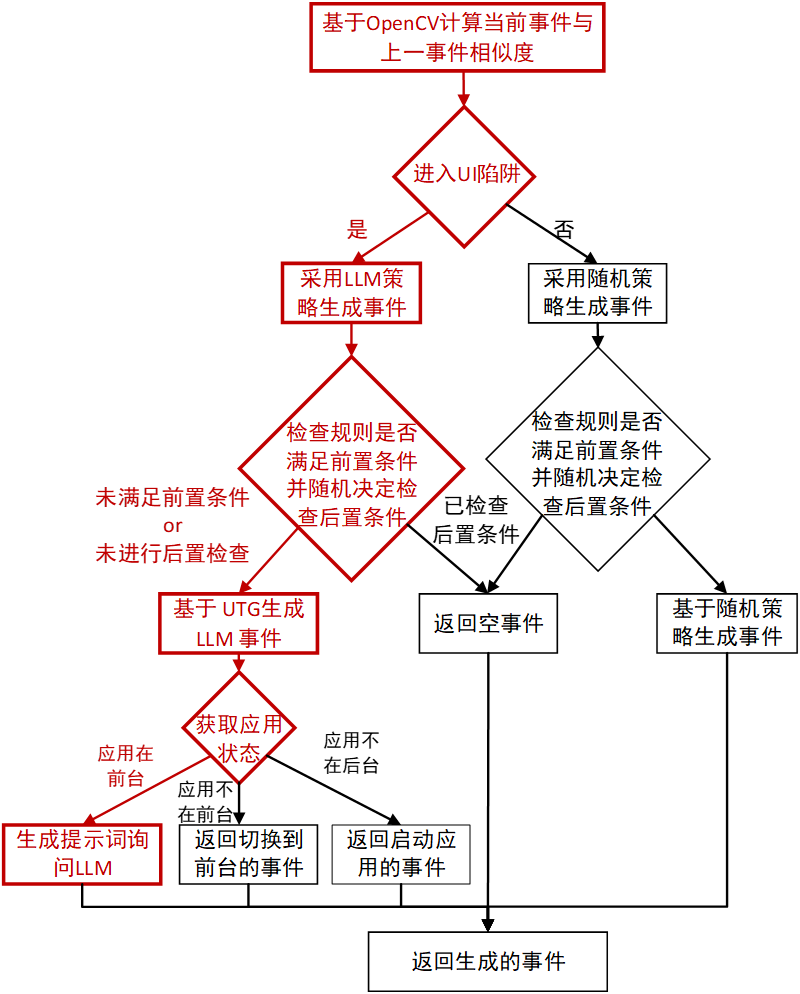
\includegraphics[width=0.5\textwidth]{llm}
    \caption{\kea 现有的大模型引导策略示意图,红色框线图示了触发大模型引导策略的执行过程。}
    \figureBelowMargin
    \label{fig:llm}
\end{figure}

\kea 目前提供了三种路径探索策略:随机探索、主路径引导探索、和大语言模型辅助的探索。其中,随机探索策略随机地生成输入事件序列,主路经引导探索策略在用户指定的应用``主路径''附近进行随机探索。

大语言模型引导策略(LLM策略)则是对随机策略的加强,主要负责在应用状态空间中遇到难以探索的UI状态时,利用 LLM 生成输入事件以增强功能场景覆盖。具体来讲,该策略在随机探索的基础上,于每次输入事件生成前检测当前的UI状态是否处于UI陷阱(即UI tarpit,``焦油坑''\cite{khan2024aurora})。若处于UI陷阱,则使用大语言模型生成输入事件,试图跳出UI陷阱。

然而,\kea 现有的大语言模型引导策略仍存在一些不足。我们实验观察中发现,在某些情况下,LLM生成的操作序列仍可能无法有效跳出当前状态,导致陷入死循环或无响应状态。我们将在后续进行分析。

\section{问题}

现有的LLM策略主要分为相似度检测和生成事件两个模块。图 \ref{fig:llm} 展示了现有的大模型引导策略的基本流程。

进行相似度检测时,\kea 采用了 OpenCV 来对比两个连续的UI状态的屏幕截图,从而计算两个状态之间的相似度,当连续多次相似度超过设定的阈值时,\kea 认为当前处于UI陷阱。此时,\kea 会使用大语言模型生成输入事件,试图跳出UI陷阱。基于现有的UI状态信息和可能的输入事件,\kea 会询问大语言模型,由大语言模型给出一个输入事件并执行。

\begin{figure}[t]
    \centering
    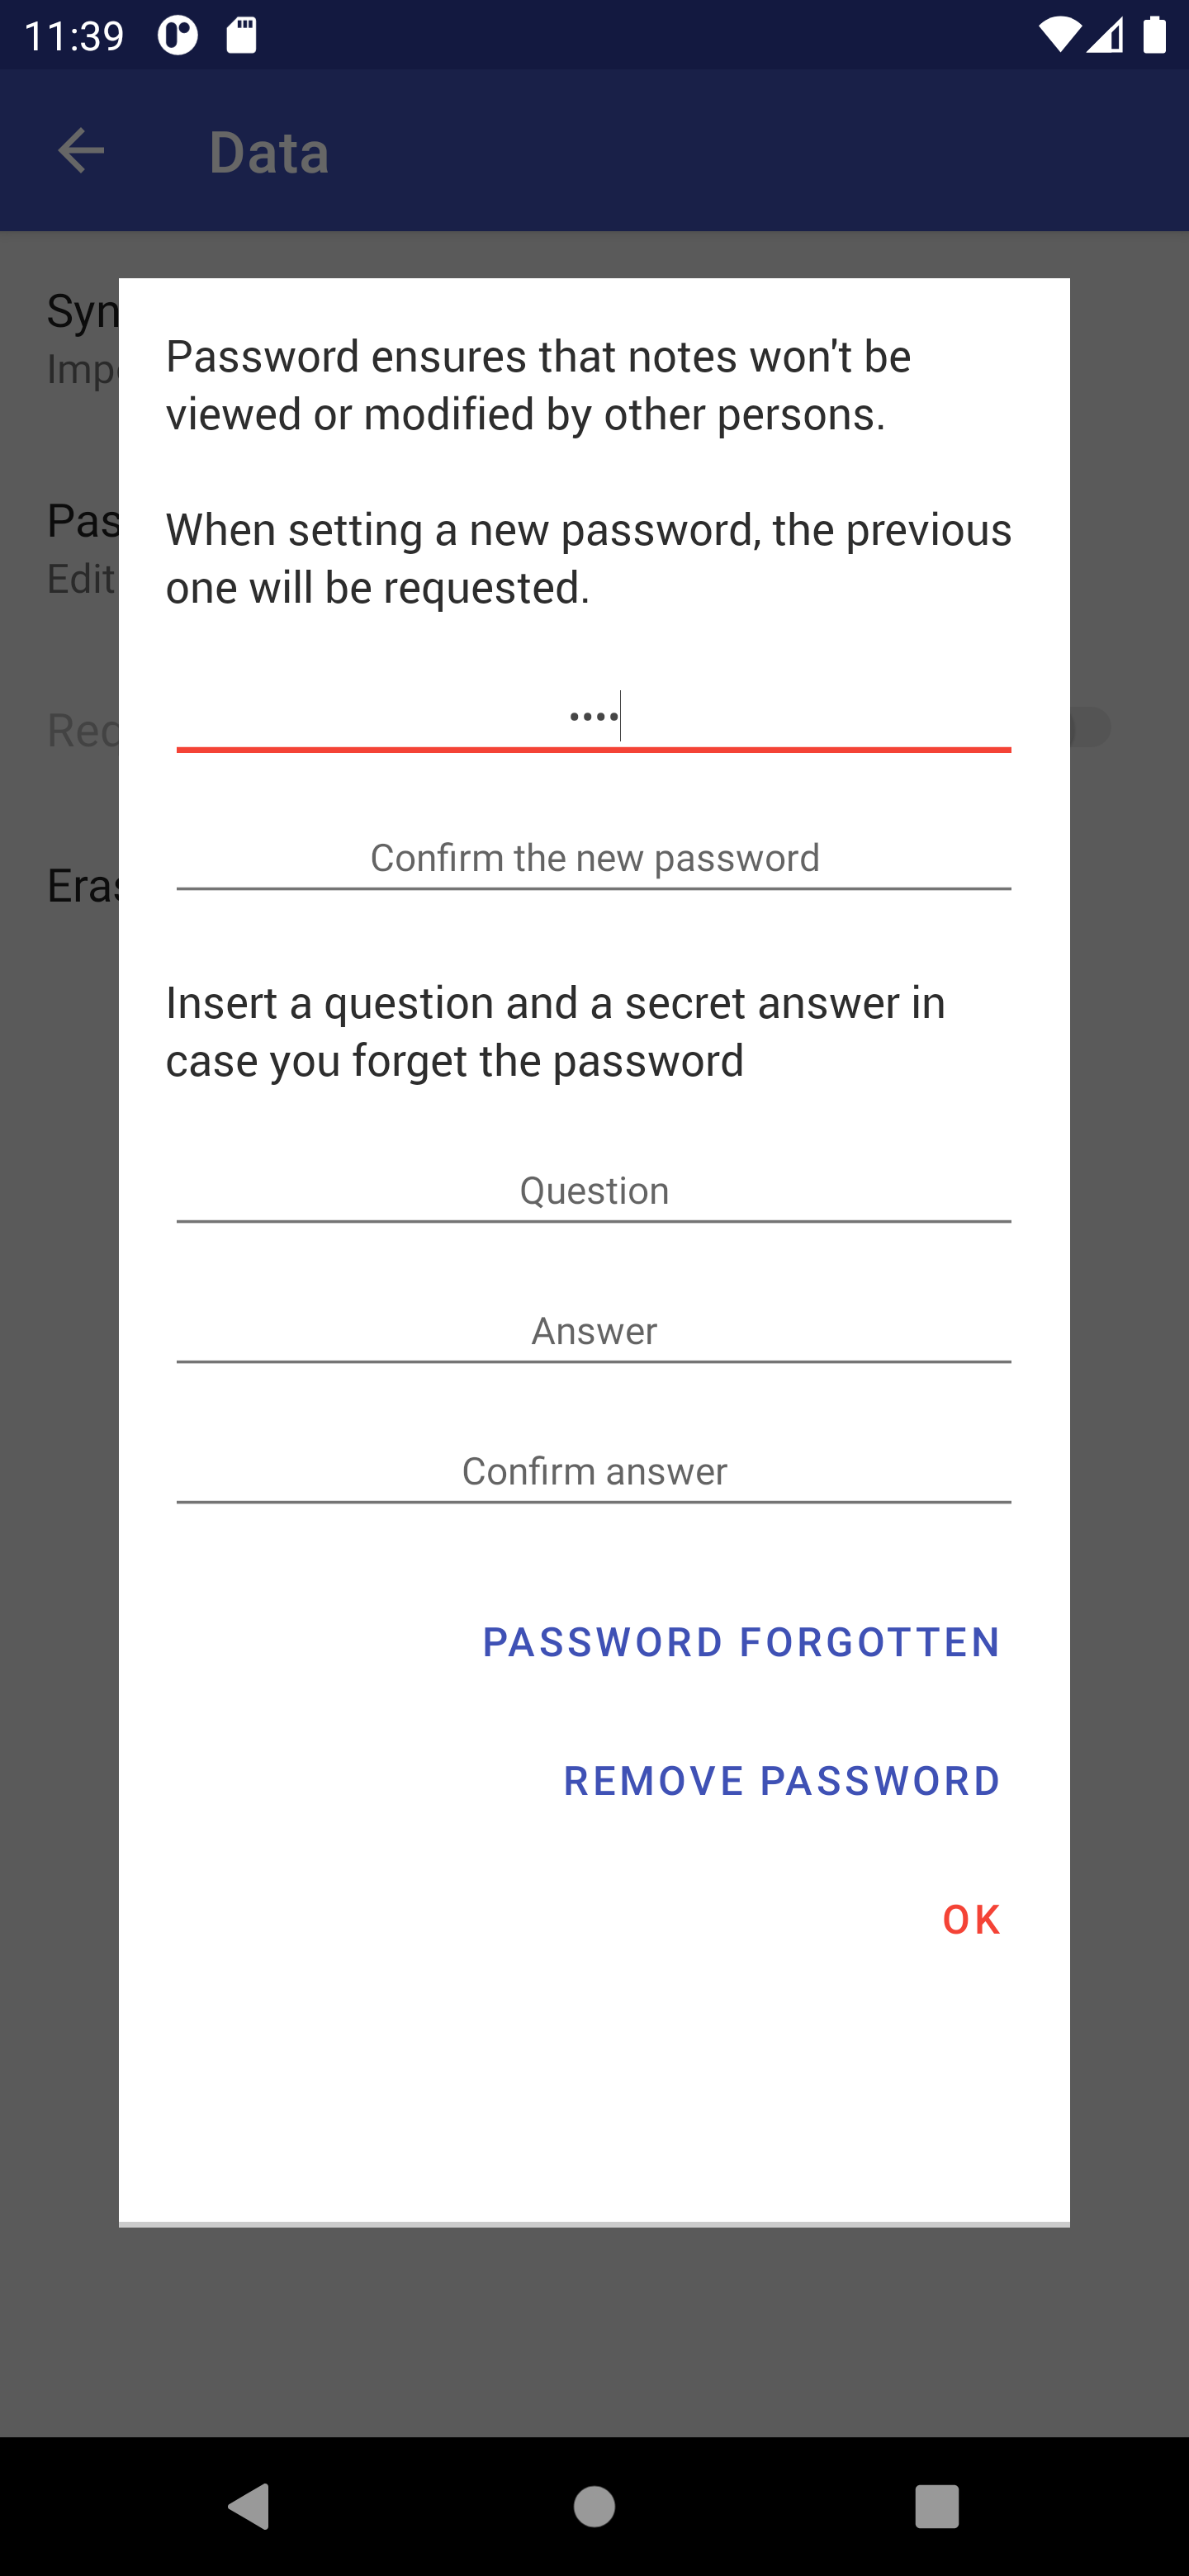
\includegraphics[width=0.3\textwidth]{1}
    \caption{Omni-Notes应用的UI陷阱示例}
    \label{fig:omni_tarpit}
\end{figure}


\begin{figure}[ht!]
    \centering
    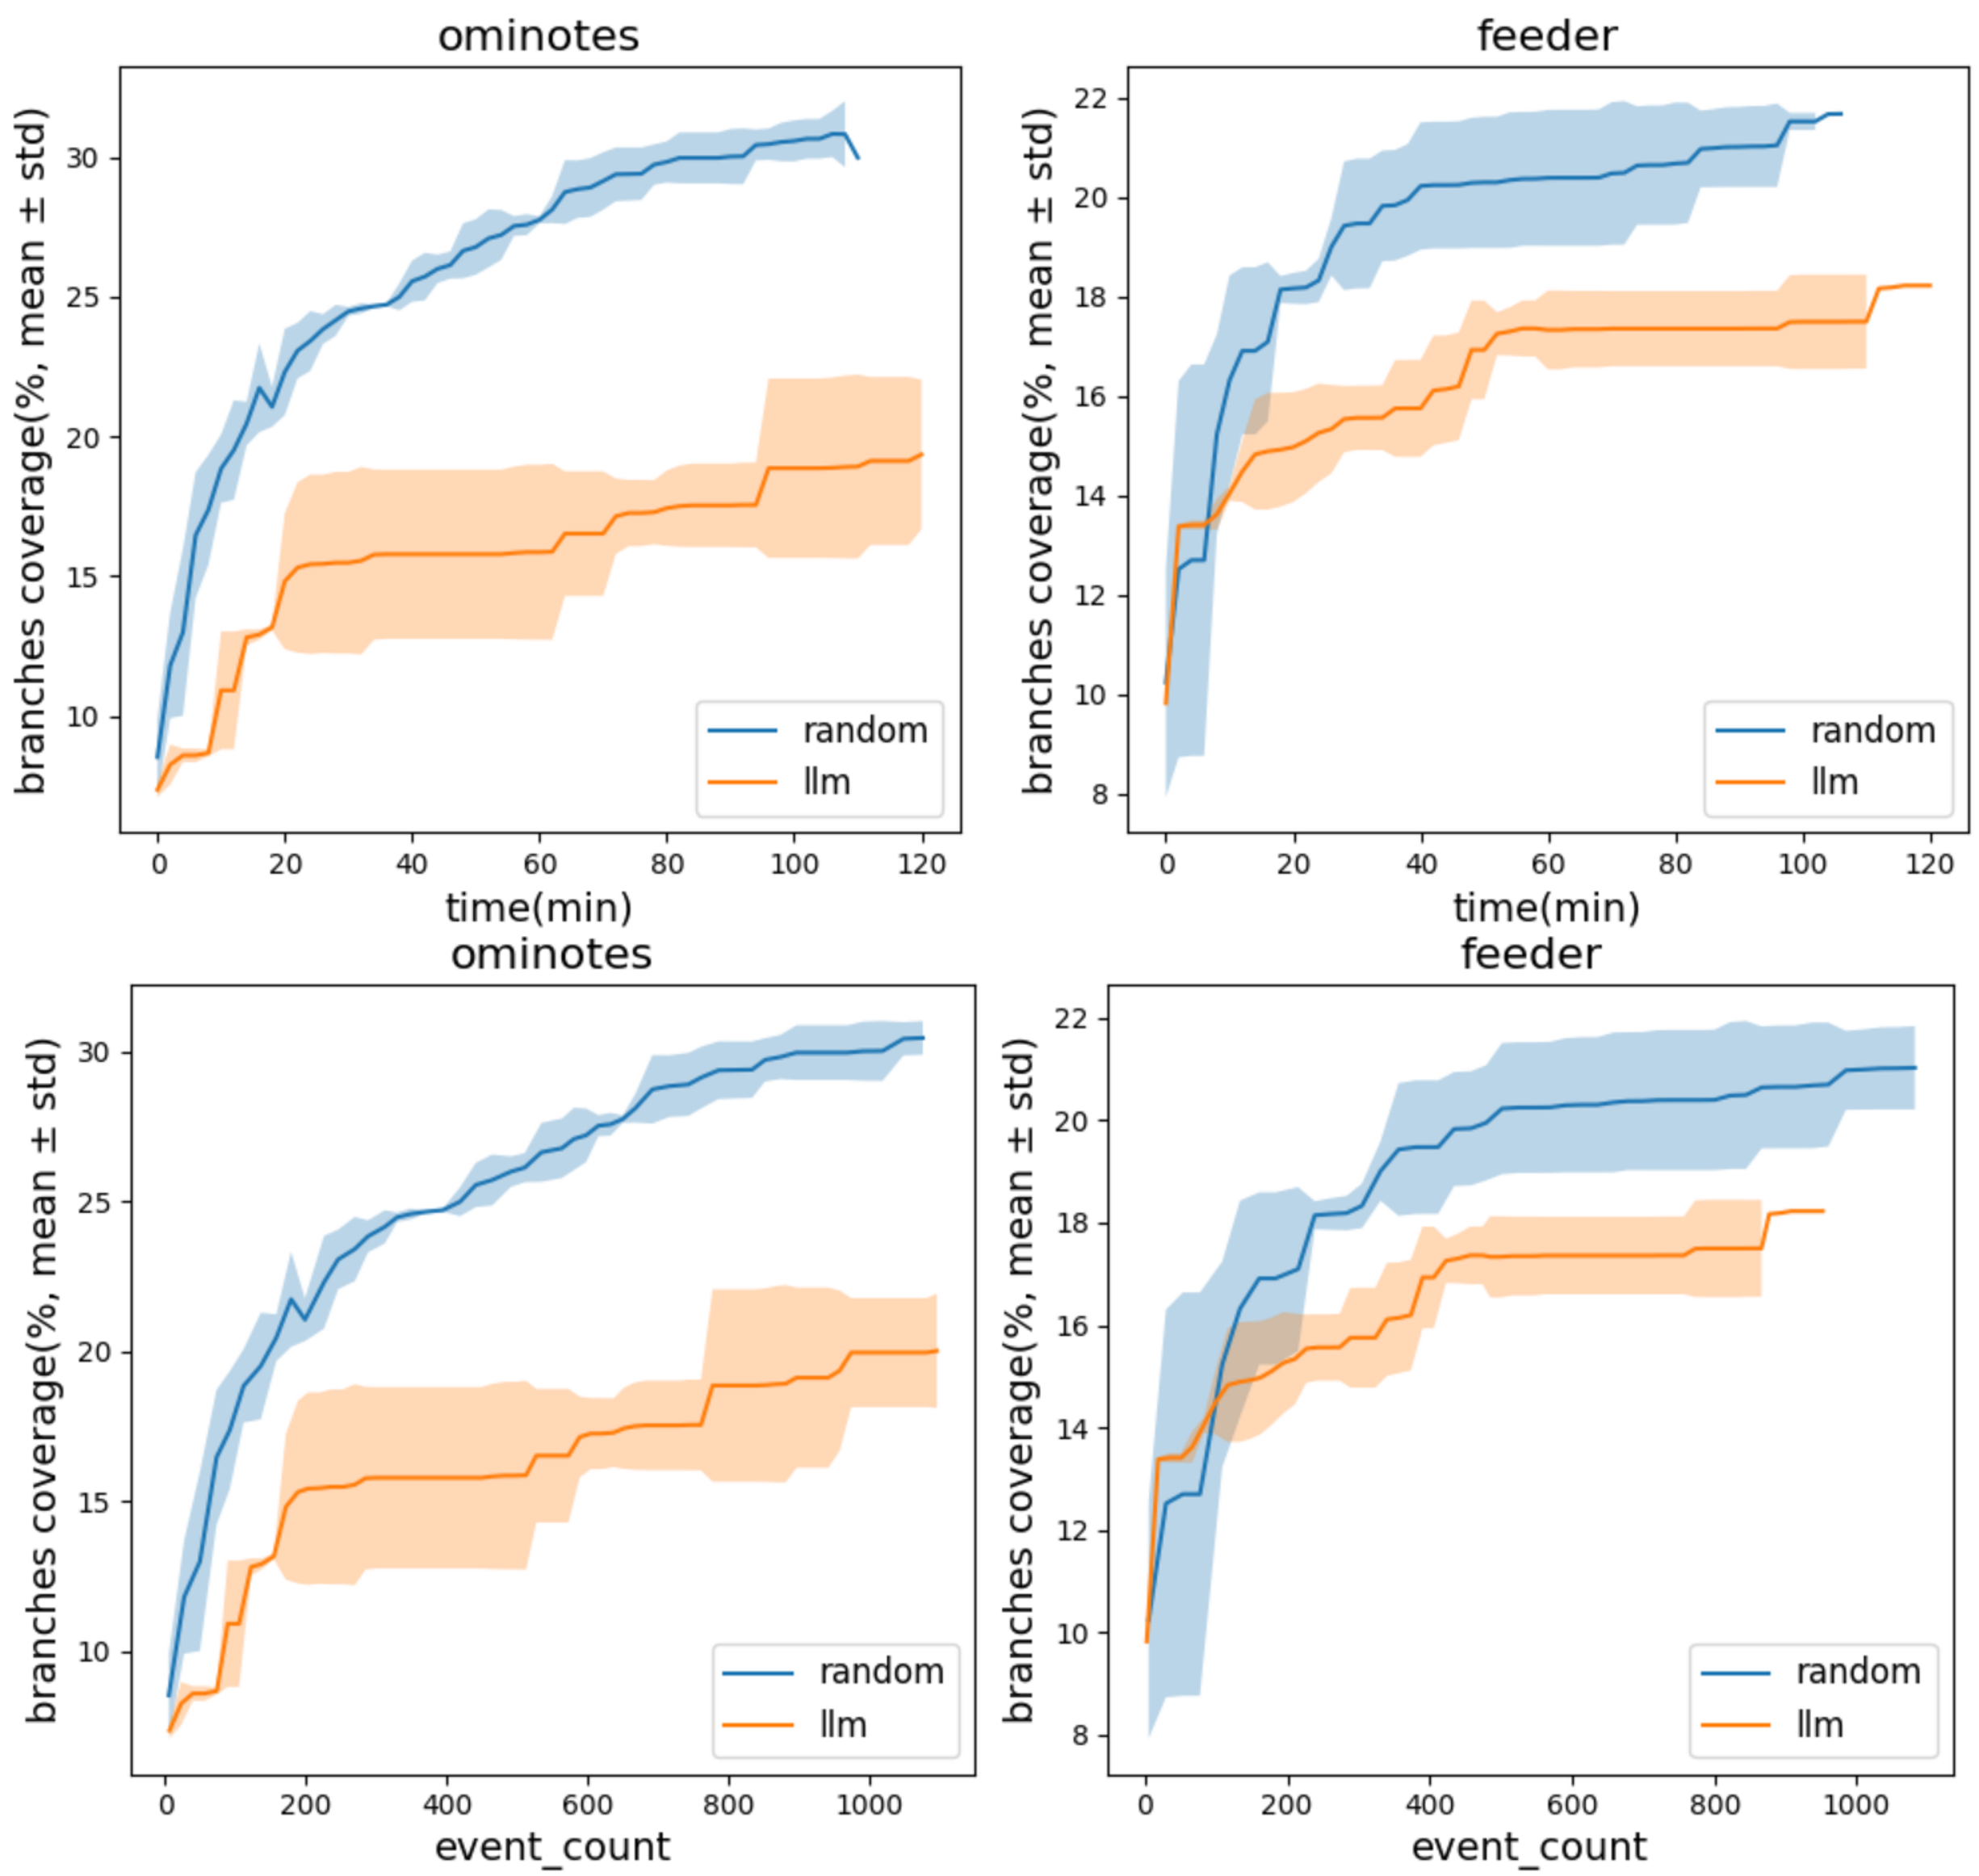
\includegraphics[width=0.5\textwidth]{llm_test}
    \caption{LLM策略和随机策略相同时间或相同事件数量时代码分支覆盖率,阴影表示三次实验的标准差。}
    \label{fig:llm_test}
\end{figure}

然而,现有LLM策略效果不佳。如图 \ref{fig:omni_tarpit} 所示,该界面是Omni-Notes的笔记密码设置页面,用户必须在填写表单后才能点击按钮进行跳转。在随机探索的策略下,\kea 会陷入死循环,无法有效地跳出该页面。当我们使用\kea 现有的 LLM 策略时,发现生成的输入事件仍然无法有效地跳出该页面,导致长期在该页面陷入死循环。这主要是因为,当前 LLM 策略选择的输入事件仅依赖于当前UI状态下可执行的输入事件。LLM 并不能理解当前UI状态下的界面结构,缺乏对页面上组件信息的深入理解,使其生成的操作不够准确。同时,LLM 策略所生成的输入事件并不依赖于以往的输入事件序列,缺乏上下文感知能力。即,LLM 生成的输入事件$\phi_i$的生成仅依赖于当前UI状态$\theta_i$,却无法感知 LLM 之前的输入事件所形成的事件序列$\{\phi_1, \phi_2, \ldots, \phi_{i-1}\}$的\textbf{真实意图}。这使得 LLM 策略在生成输入事件时缺失了对核心任务的理解,从而导致生成的输入事件不够准确。这些问题都导致了 LLM 策略在跳出UI陷阱时的效果不佳。

同时,我们在实验过程中发现,两种情况会导致 LLM 策略产生导致显著的额外开销:1) LLM 策略可能会生成无效操作,生成的输入事件并不能逃离UI陷阱;2) 现有的相似度检测方法可能会导致UI陷阱误判。在这些情况下,LLM 策略会频繁地调用大语言模型来生成输入事件,消耗了 LLM 资源和通信时间。

图 \ref{fig:llm_test} 展示了运行LLM策略和随机策略相同时间或相同事件数量时的代码分支覆盖率,LLM策略相比随机策略不但没有提升,甚至有所明显的下降。(如,Omni-Notes中,分支覆盖率平均下降了39.31\%)

总而言之,现有策略存在的三个问题:\textbf{1) LLM 策略在解决 UI 陷阱方面效果不佳,其生成的事件不准确,且缺乏上下文感知能力;2) LLM 策略由于需要频繁调用,会产生显著的调用开销;3) 现有的相似度检测方法可能会导致误判。}

因此,我们提出了一种新的大语言模型辅助的路径探索策略,称为\lamp(Large-language-model Augmented Mobile Testing Path Exploration Based on \kea)。\lamp 通过引入基于语义的UI陷阱检测算法和基于迭代事件序列生成 的增强型LLM探索策略,结合大语言模型的语义理解和生成能力,提升了路径探索的效率和准确性。

\section{方法}

我们提出了三种方法来优化现有的 LLM 策略。在\textsection~\ref{sec:semantic}中,我们提出了一种基于语义的 UI 陷阱检测算法,利用 UI 界面的 XML 语义结构来判断 UI 陷阱;在\textsection~\ref{sec:iterative}中,我们提出了一种基于迭代事件序列生成的增强型 LLM 探索策略,采用循环迭代的方式来逐步引导大语言模型生成操作序列,从而模拟人类操作的思维过程;在\textsection~\ref{sec:frequency}中,我们提出了一种频率感知的随机探索策略,通过缓存输入事件的触发频率来优化路径探索。其余的贡献在

\subsection{基于语义的UI陷阱检测算法}
\label{sec:semantic}

\begin{algorithm}[t]
\caption{Detect UI Tarpit}
\label{alg:detect_tarpit}
\begin{algorithmic}[1]
\Function{Detect}{$xml_1$, $xml_2$, $threshold$}
    \State $similarity$ $\gets$ \Call{CompareXML}{$xml_1$, $xml_2$}
    \If{$similarity$ $>$ 90}
    \State $sim\_count$ $\gets$ $sim\_count$ + 1
    \If{$sim\_count$ $\geq$ $threshold$}
        \State $sim\_count$ $\gets$ 0
        \State \Return \textbf{True}
    \EndIf
\EndIf
\State \Return \textbf{False}
\EndFunction
\end{algorithmic}
\end{algorithm}

\begin{algorithm}[t]
\caption{Compare XML}
\label{alg:compare_xml}
\begin{algorithmic}[1]
\Function{CompareXML}{$xml_1$, $xml_2$}
    \State $tree_1, tree_2 \gets$ Simplify $xml_1$, $xml_2$ and construct trees
    \State $score, total \gets \Call{CompareTree}{tree_1, tree_2}$
    \State \Return $100.0$ if $total = 0$ else $(score / total) \times 100$
\EndFunction
\end{algorithmic}
\end{algorithm}

\begin{figure}[t]
    \centering
    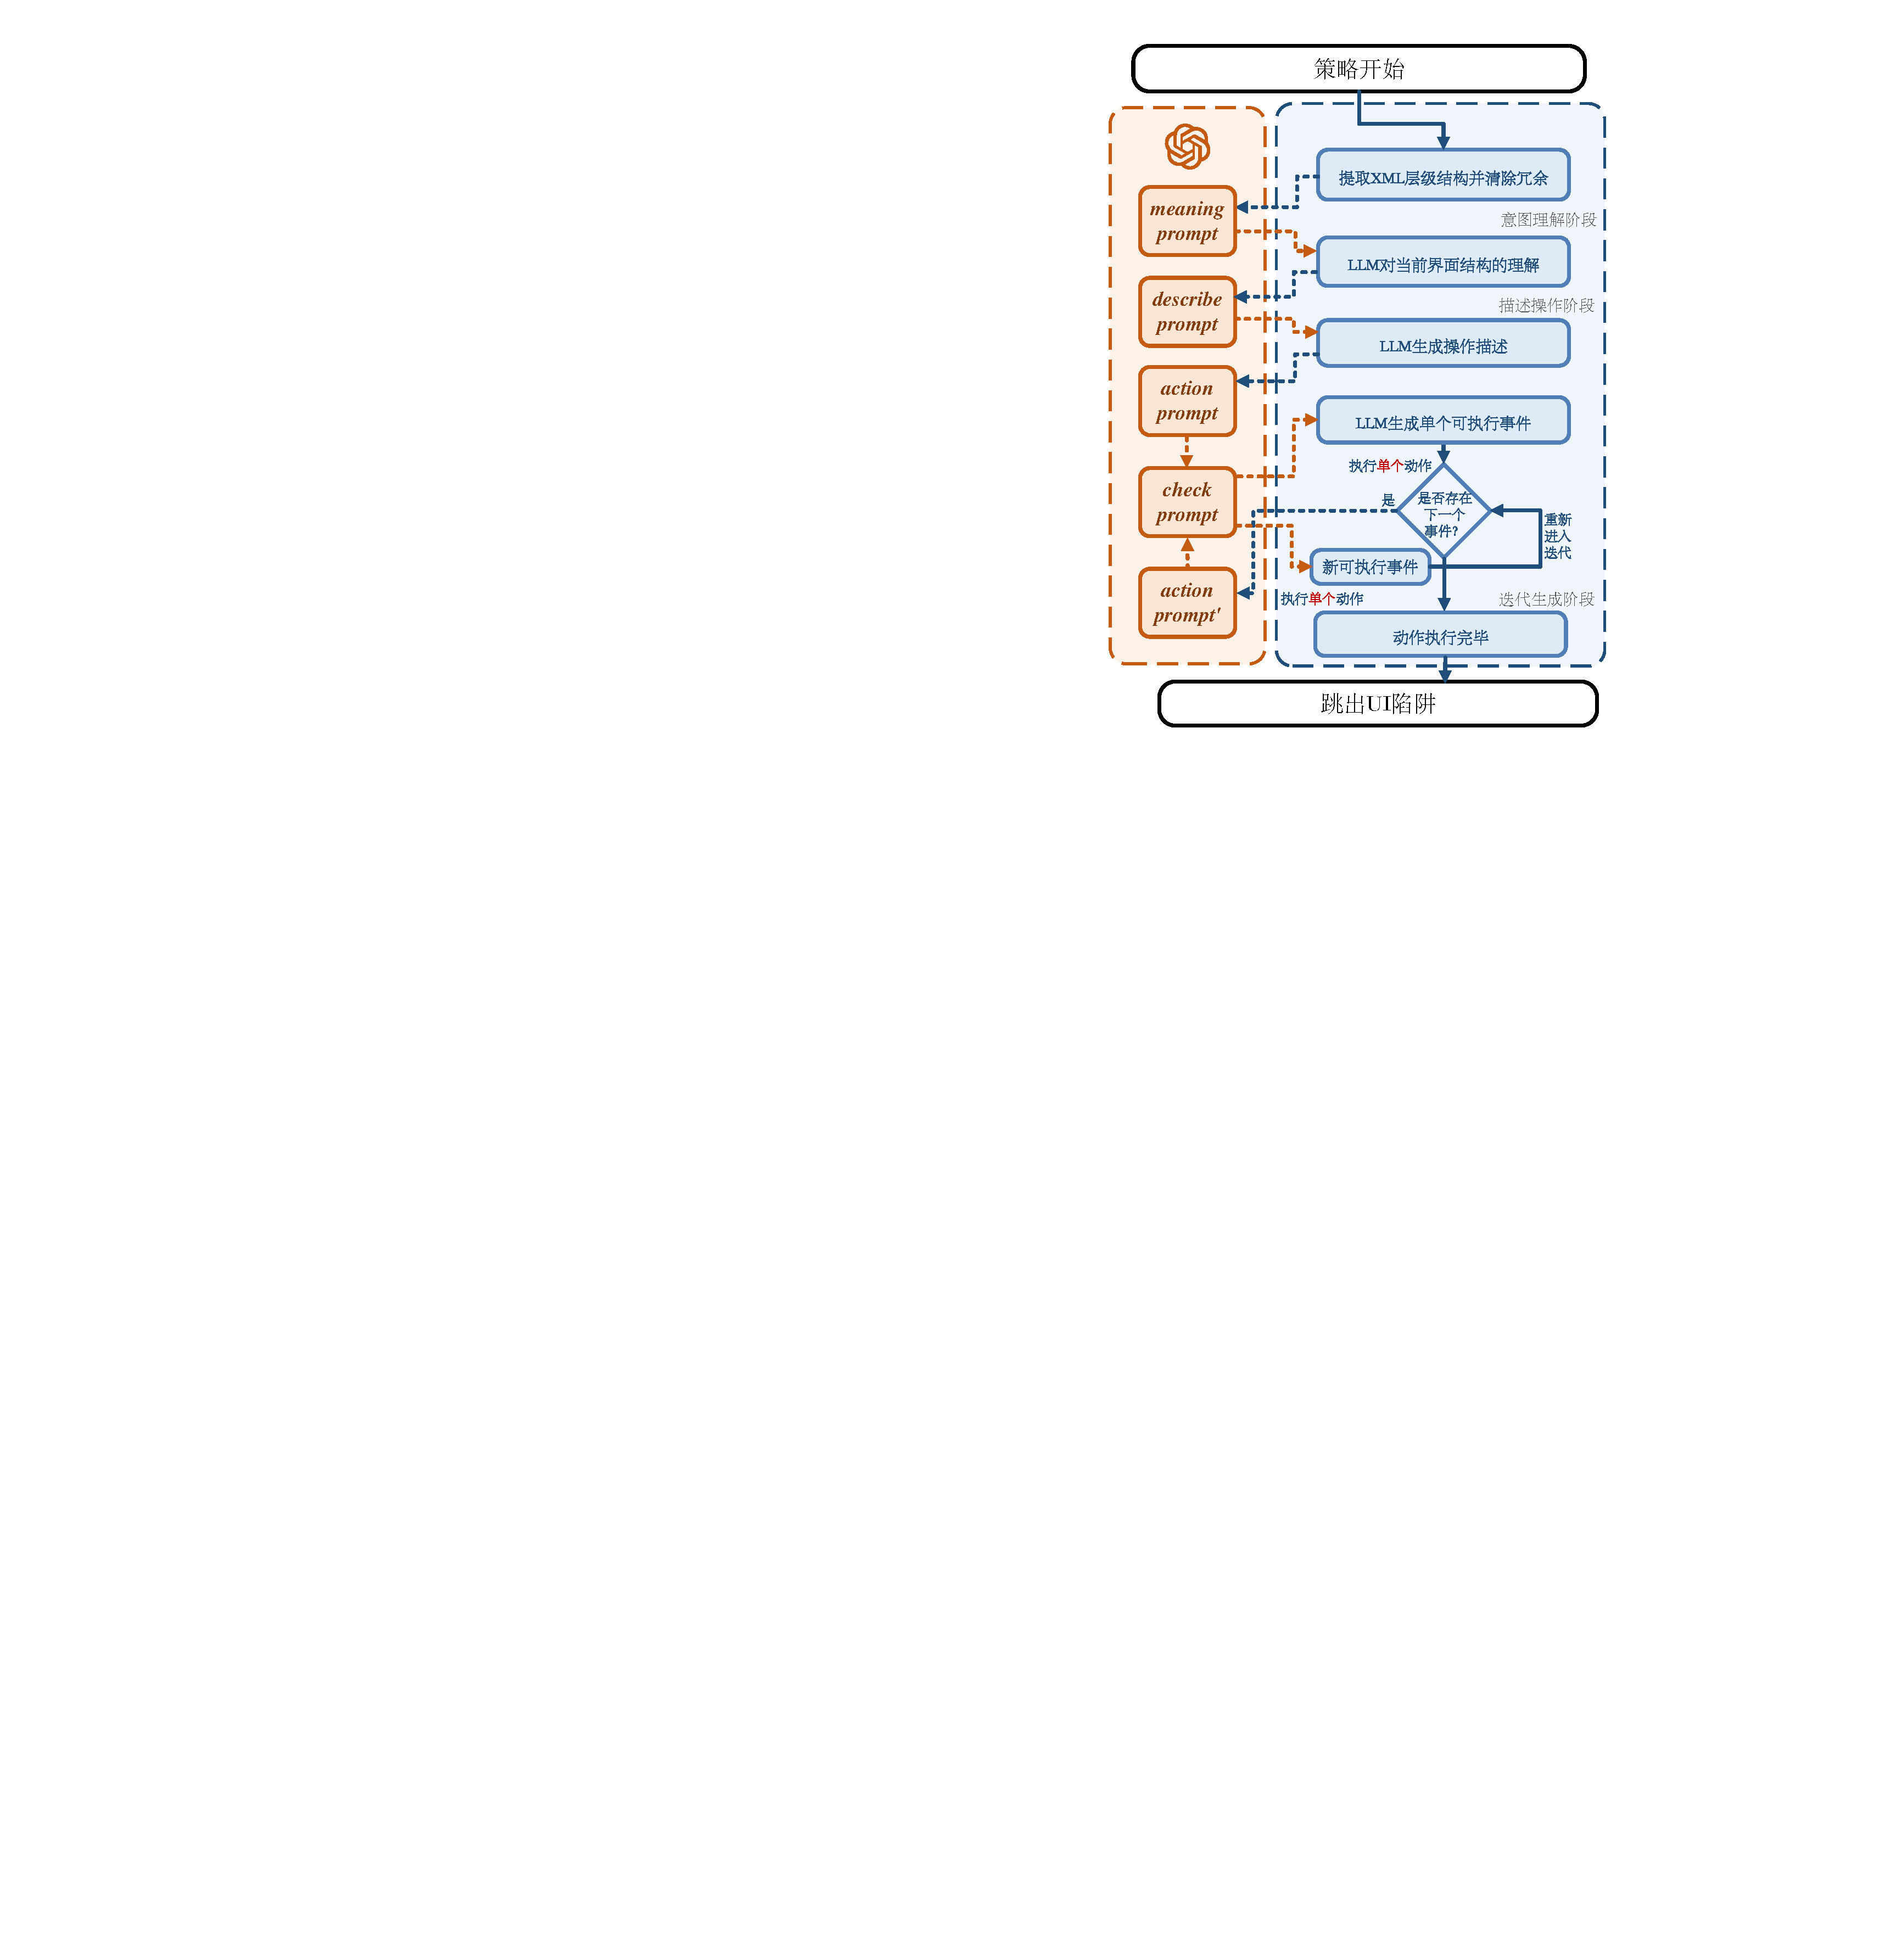
\includegraphics[width=0.4\textwidth]{pic}
    \caption{基于迭代的提示工程}
    \label{fig:process}
\end{figure}

我们在 \kea 的 LLM 策略原有的相似度计算方案的基础上,重新提出了一种新的相似度计算方案,希望通过关注 UI 界面的 XML 语义结构来判断 UI 陷阱。我们发现, XML 树结构能够更好地反映 UI 状态的语义信息和层次关系,因此可以通过对比两个 UI 状态的 XML 树结构,来判断两个UI 状态是否相似。

为此,我们将 XML 树结构进行简化,将 XML 树抽象成只包含 tag 和 children 的轻量结构,便于对结构相似性进行对比。如算法~\ref{alg:compare_xml}所示,我们得到了两个简化后的 XML 树结构 $tree_1$ 和 $tree_2$,然后通过调用\texttt{CompareTree}函数递归遍历树结构,计算两个树的相似度分数 $score$ 和总节点数 $total$。最后,我们返回相似度分数。

随后,在算法~\ref{alg:detect_tarpit}中,我们沿用了 \kea 的 LLM 策略原有的启发式相似度判断方案,使用 \texttt{CompareXML} 函数来计算两个 UI 状态的相似度分数 $similarity$后,如果相似度分数大于 90,则认为两个 UI 状态相似。我们使用一个计数器 $sim\_count$ 来记录连续相似的次数,当连续相似的次数超过设定的阈值时,我们认为当前处于 UI 陷阱。

在后续的测试过程中我们观察到,该方法显著减少了对 UI 陷阱的误判,同时仍能够识别出原有相似度检测方法所发现的 UI 陷阱。经过人工验证,这些 UI 陷阱确实是难以被探索的 UI 状态。这样的方法提高了 LLM 策略的效率,减少了对大语言模型的调用次数。

\subsection{基于迭代事件序列生成的增强型LLM探索策略}
\label{sec:iterative}

我们将提示工程包括三个阶段:1)\textbf{意图理解阶段}(\textsection~\ref{sec:intent});2)\textbf{操作描述阶段}(\textsection~\ref{sec:action});3)\textbf{迭代生成阶段}(\textsection~\ref{sec:iterative_generate})。我们在\textsection~\ref{sec:generate_event}中介绍了整个 LLM 事件生成的算法流程。流程图如图\ref{fig:process}所示。

\subsubsection{意图理解阶段}
\label{sec:intent}

在这一阶段,我们将获取到的XML结构作为上下文输入到大语言模型中,要求其理解当前界面的意图和功能。但是,由于通过 \texttt{uiautomator2} 获取的XML结构内容比较复杂,通常含有大量无用和干扰信息。因此,我们首先对XML数据进行预处理。首先,我们去除了XML中系统状态栏的结构信息,以减少干扰。其次,我们删除了值为空字符串和 \texttt{false}的属性,以精简XML,减少无用信息。

我们设计了一个提示词 \texttt{meaning\_prompt()}(见附录~\ref{sec:prompt}),用于引导模型生成对当前界面的描述。通过获取到模型对当前界面结构的理解,我们可以更好地引导模型生成后续的操作序列。

\subsubsection{操作描述阶段}
\label{sec:action}

在这一阶段,我们根据之前的上下文信息,向大语言模型提出新的要求——要求其生成一个完整任务流程的描述,从而引导模型一步步生成事件。

我们设计了一个提示词 describe\_prompt(见附录~\ref{sec:prompt}),用于引导大语言模型基于当前UI页面生成一个用户可能执行的新操作。该提示词明确要求模型仅描述一个尚未生成的任务,并补充执行该任务所需的具体步骤,从而在一定程度上避免了重复。此外,提示中加入了当前已生成任务的列表,进一步实现了去重,引导模型从\textbf{用户视角}出发进行交互意图推理。

\begin{algorithm}[t]
\caption{Main Exploration Loop}
\label{alg:main}
\begin{algorithmic}[1]
\Function{Start}{${input\_manager}$}
  \State $count \gets 0$
  \While{$count < max\_event\_count$}
    \State Update UI state and snapshots
    \State Start the APP if essential
    \If{LLM mode is active}
        \State $event \gets$ \Call{GenerateLLMEvent}{}
    \ElsIf{\Call{DetectUITarpit}{$last\_state$, $current\_state$}}
        \State Activate LLM Mode
        \State $event \gets$ \Call{GenerateLLMEvent}{}
    \Else
        \State $event \gets$ \Call{GenerateRandomEvent}{}
    \EndIf
    \State \Call{Execute}{$event$}
    \State $count \gets count + 1$
  \EndWhile
  \State Clean up and exit
\EndFunction
\end{algorithmic}
\end{algorithm}

\begin{algorithm}[t]
\caption{Generate LLM Event}
\label{alg:generate_event}
\begin{algorithmic}[1]
\Function{GenerateLLMEvent}{}
    \If{Continuing LLM Sequence}
          \State Build Next Action Prompt
          \State $response \gets$ \Call{CallLLM}{}
          \State $response \gets$ \Call{ValiditeByLLM}{}
          \State $act \gets$ \Call{ParseAction}{$response$}
        \Else
          \State Build Meaning Prompt
          \State $r_1 \gets$ \Call{CallLLM}{}
          \State Build Task Prompt
          \State $r_2 \gets$ \Call{CallLLM}{}
          \State Build First Action Prompt
          \State $r_3 \gets$ \Call{CallLLM}{}
          \State $response \gets$ \Call{ValiditeByLLM}{}
          \State $act \gets$ \Call{ParseAction}{$response$}
    \EndIf
    \State Set LLM Mode to $act.hasNext$
    \State \Return \Call{WrapAsU2Event}{act}
\EndFunction
\end{algorithmic}
\end{algorithm}

\subsubsection{迭代生成阶段}
\label{sec:iterative_generate}

在这个阶段中,我们将大语言模型生成的操作描述作为输入,不断要求模型生成新的操作序列。我们设计了两个提示词 action\_prompt 和 action\_prompt\_prime(见附录~\ref{sec:prompt}),分别用于引导模型生成操作序列的第一步和后续步骤。

在 action\_prompt 中,我们引导大语言模型将用户操作步骤以结构化的 JSON 格式进行表达,以便于后续被程序解析与执行。该提示词强调只描述“用户刚刚执行的操作的第一步”,并提供了统一的格式规范和字段说明,如 action、selectors、inputText 和 hasNext。其中,selectors 用于精确定位页面元素,支持多种常见属性组合(如 resourceId 与 text),并要求所有值必须可在对应的 UI XML 中找到,以确保操作的可执行性与准确性。此外,通过布尔值 hasNext,我们可以判断是否还有后续操作需要生成。

在 action\_prompt\_prime 中,我们引导大语言模型在给定当前页面状态的基础上,继续生成前一个操作的“下一步”操作。该提示词通过动态插入最新的页面 XML 状态,确保模型具备当前 UI 上下文,从而做出合理的操作。

在生成操作序列后,我们还需要对生成的操作进行检查,以确保其符合要求。我们设计了一个提示词 check\_prompt(见附录~\ref{sec:prompt}),用于引导大语言模型检查生成的操作是否符合要求。该提示词要求模型检查生成的操作是否符合以下两个条件:1)选择器必须在 XML 中找到;2)选择器必须唯一标识元素。如果没有问题,则按原样输出;否则,修改相应内容。

\subsubsection{事件生成流程}
\label{sec:generate_event}

如算法~\ref{alg:main}所示,系统在主循环中不断执行事件生成与执行流程。每轮循环中,系统会根据当前状态选择事件生成策略:当 LLM 模式处于激活状态时,调用 \texttt{GenerateLLMEvent()} 函数生成由大语言模型驱动的操作事件;否则,将调用 \texttt{GenerateRandomEvent()} 函数生成随机事件。若系统检测到 UI 陷阱(UI Tarpit),也会触发 LLM 模式并转为基于模型的操作生成。

算法~\ref{alg:generate_event}展示了 \texttt{GenerateLLMEvent()} 函数的内部逻辑。函数首先判断是否正在延续一个 LLM 操作序列:若是,则调用 \texttt{BuildNextActionPrompt()} 构造提示,获取 LLM 响应,并依次通过 \texttt{ValiditeByLLM()} 验证响应有效性,再调用 \texttt{ParseAction()} 解析出具体操作;否则,将按顺序构建页面意图、任务目标和首个动作的提示,分别调用 \texttt{CallLLM()} 获取响应,最终进行验证和解析操作。最后,该函数会根据操作是否存在后续步骤(\texttt{hasNext})来更新 LLM 模式,并将解析结果包装为 U2 可执行事件返回。

\begin{algorithm}[t]
\caption{Frequency-Aware Random Strategy}
\label{alg:random}
\begin{algorithmic}[1]
\Function{GenerateEvent}{}
\State $s \gets$ current state
\If{$s \notin input\_table$}
    \State $possible\_events \gets \Call{GetPossibleInputs}{s}$
    \State Initialize $input\_table[s]$ with an empty \texttt{events} list
    \ForAll{$event \in possible\_events$}
        \State Add $event$ to $input\_table[s].events$
        \If{$event \notin event\_table$}
            \State $event\_table[event] \gets$ 0
        \EndIf
    \EndFor
\EndIf
    \State $counts$ $\gets$ $\emptyset$
    \ForAll{$event \in input\_table[s].events$}
        \State $counts[event] \gets event\_table[event].tried$
    \EndFor
    \State $weights \gets$ \Call{GetWeights}{$input\_table[s].events$, $counts$}
    \State $selected\_event \gets$ randomly select one event from the list using $weights$
    \State Increment $event\_table[selected\_event].tried$
    \State \Return $selected\_event$
\EndFunction
\end{algorithmic}
\end{algorithm}

\subsection{频率感知的随机探索策略}
\label{sec:frequency}

我们提出了一种频率感知的随机探索策略(见算法~\ref{alg:random}),通过记录和利用输入事件的触发频率,引导探索过程更均匀地覆盖不同事件,避免某些操作被频繁重复触发。

在事件生成过程中,系统首先检查当前状态是否已存在于 \texttt{input\_table} 中。若不存在,则通过 \texttt{GetPossibleInputs} 获取该状态下所有可能的输入事件,并将其记录在 \texttt{input\_table} 中。对于每个新事件,如果其尚未存在于 \texttt{event\_table} 中,系统会初始化其尝试次数为零。

随后,系统统计当前状态下各输入事件的触发频次,从 \texttt{event\_table} 中获取每个事件的尝试次数,并根据这些频率计算采样权重(通过 \texttt{GetWeights} 函数)。最终,系统根据权重随机选择一个输入事件,并更新其尝试次数,用于执行。

为了避免重复选择已经尝试过的事件,又要防止尝试过的事件完全被忽略,我们设计了一种基于频率的采样方法 \texttt{GetWeights} 函数。设 $E = \{e_1, e_2, \dots, e_n\}$ 为所有可能事件的集合,令 $c_i$ 表示事件 $e_i$ 已被尝试的次数。给定一个衰减因子 $\gamma \in (0, 1)$,选择事件 $e_i$ 的权重 $w_i$ 可以表示为:

\begin{equation}
    w_i = w_0 \cdot \gamma^{c_i}
\end{equation}

因此,事件 $e_i$ 被选择的概率 $P(e_i)$ 可以表示为:

\begin{equation}
    P(e_i) = \frac{w_i}{\sum_{j=1}^{n} w_j} = \frac{\gamma^{c_i}}{\sum_{j=1}^{n} \gamma^{c_j}}
\end{equation}

通过采用指数衰减的方式,我们可以有效地平衡新事件和已尝试事件的选择概率,从而实现更均匀的探索。

\section{实验}

\subsection{实验设置}
\label{sec:setup}

\subsubsection{数据集}

\begin{table}[t]
\small
\centering
\caption{本文使用的应用数据集}
\label{tab:app-dataset}
\begin{tabular}{@{}llll@{}}
\toprule
\textbf{App}    & \textbf{Primary Feature}        & \textbf{Stars} & \textbf{Installations} \\ 
\midrule
AnkiDroid   & Flashcard Manager     & 9.5K         & 10M–50M       \\
Feeder      & RSS Feed Reader        & 2.1K         & 100K–500K     \\
Newpipe     & YouTube Client         & 33.8K        & 1M–5M         \\
OmniNotes   & Note Manager           & 2.7K         & 10M–50M       \\
Wikipedia   & Wiki Reader    & 3K           & 10M–50M       \\
\bottomrule
\end{tabular}
\end{table}


\subsubsection{实验环境}




\appendix

\section{提示工程}
\label{sec:prompt}

\begin{itemize}
    \item 意图理解:见代码~1。
    \item 操作描述:见代码~2。
    \item 迭代生成:见代码~3。
    \item 后续事件生成:见代码~4。
    \item 操作检查:见代码~5。
\end{itemize}

\begin{figure*}[t]
\centering
\begin{lstlisting}[language=Python,caption=意图理解]
    prompt = f"""This is an XML representation of an Android application page:
    {get_xml()}
    Please describe the purpose of this page in the most concise language possible."""
\end{lstlisting}
\label{fig:intent}
\end{figure*}

\begin{figure*}[t]
\centering
\begin{lstlisting}[language=python, caption=操作描述]
    prompt = f"""If you were the user, what would you do on this page? You can only describe one action. 
    Please try to generate tasks that have not been generated before. Below are the tasks that have already been generated:
    {list(self._generated_tasks)}
    Please list the steps required to complete this action. (This action will be named 'The Task')"""
\end{lstlisting}
\label{fig:action}
\end{figure*}

\begin{figure*}[t]
\centering
\begin{lstlisting}[language=python, caption=初始事件生成]
    prompt = """Please describe the **first step** of the operation you just performed in JSON format, as shown below:
    {
        "action": "input_text",
        "selectors": {"resourceId": "com.example:id/input", "text": "password"},
        "inputText": "123456",
        "hasNext": true
    }
    Notes:
    - The "action" must be one of: click, long_click, input_text, press_enter
    - "selectors" can only include: **text**, **className**, **description**, **resourceId**, and must be in camelCase. You can not use other selectors.
    - The value is the value of the selector, which must be found in the previous XML
    - "inputText" is the text to input, only present when the action is input_text
    - "hasNext" is a boolean indicating whether there is a next step. Set it to false if there is no next step
    Try to combine multiple selectors to uniquely identify the element.
    Please return the operation in JSON format only. Do not explain or use code blocks.
    """
\end{lstlisting}
\label{fig:iterative}
\end{figure*}

\begin{figure*}[t!]
\centering
\begin{lstlisting}[language=python, caption=后续事件生成]
    prompt = f"""Now, the current state of the page is as follows: {get_xml(self.device.u2)}
    Please describe the **next step** of the operation you just performed in JSON format, using the same format as above.
    """
\end{lstlisting}
\label{fig:next}
\end{figure*}

\begin{figure*}[t!]
\centering
\begin{lstlisting}[language=python, caption=操作检查]
    prompt = """Please check whether the operation or sequence of operations you just generated meets the requirements:
    - The selectors must be found in the XML.
    - The selectors must uniquely identify the element.
    If there are no issues, output it as is; otherwise, modify it accordingly.
    """
\end{lstlisting}
\label{fig:check}
\end{figure*}

\bibliographystyle{IEEEtran}
\bibliography{ref}

\end{document}